
\begin{frame}
    \frametitle{Cyclus Simulation of historic U.S. nuclear fuel cycle}
    \textbf{A} \textsc{Cyclus} \textbf{simulation of the U.S. nuclear fuel cycle} was created using historic United States reactor deployment data obtained from the Power Reactor Information System (PRIS) database \cite{peterson_unf_2017}.
    \\

    \textbf{Simulation Assumptions} \\
    Facilities present in the simulation: mine, mill, enrichment plant, fuel fabrication facility, 112 historic commercial reactors in the U.S, dry storage facility and a final waste repository.
    \\

    \textbf{Recipe Reactor Facility Assumptions}
    \begin{itemize}
    \item \textit{Refueling time}: 1 month
    \item \textit{Cycle length}: 18 months
    \item \textit{Single Spent Fuel Recipe}: 33 or 51 GWDt/MTU burnup (depletion calculations done using ORIGEN)
    \item \textit{Assembly size, Core size, Batch size}: dependent on the reactor type
    \item \textit{Power cap, Location}: specific to each reactor from PRIS data
    \end{itemize}
  \end{frame}

  \begin{frame}
    \frametitle{CycMap: Cyclus Simulation of historic U.S. nuclear fuel cycle}
    \begin{figure}[htbp!]
      \begin{center}
        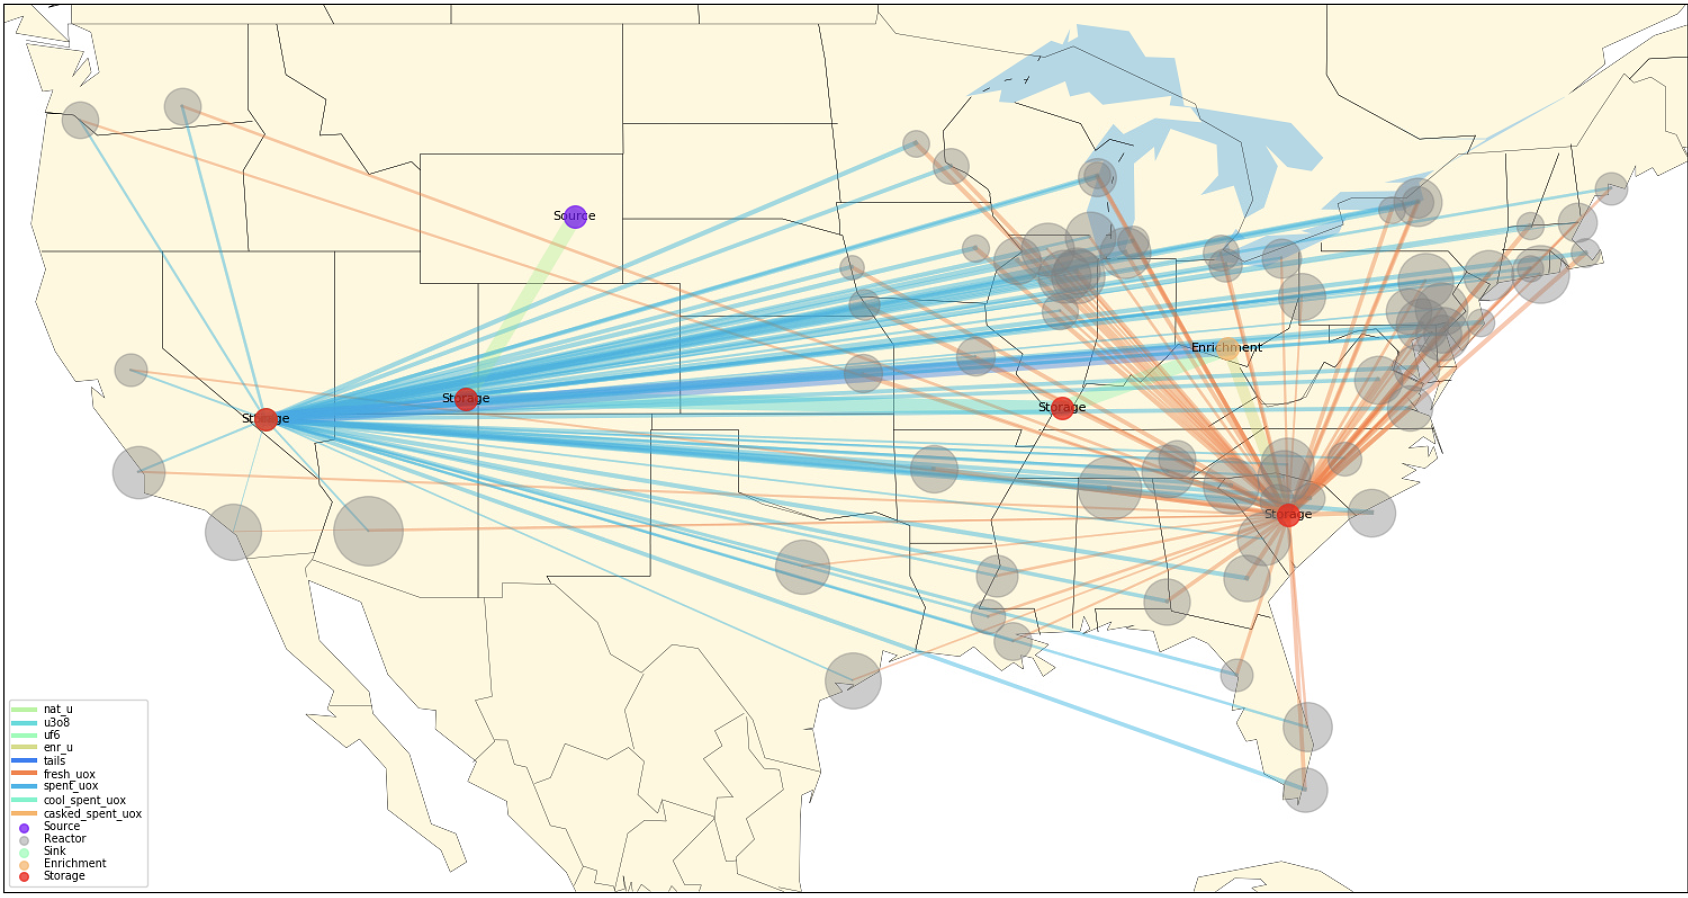
\includegraphics[height=5.5cm]{images/cycmap}
      \end{center}
            \caption{Cycmap of the historic Cyclus U.S nuclear fuel cycle simulation \cite{park_arfc/cycmap_2018}}
    \end{figure}
  \end{frame}

\begin{frame}
  \frametitle{Power demand: Cyclus Simulation of historic U.S. nuclear fuel cycle}
  \begin{columns}
    \column[t]{5cm}
    \begin{figure}[htbp!]
      \begin{center}
        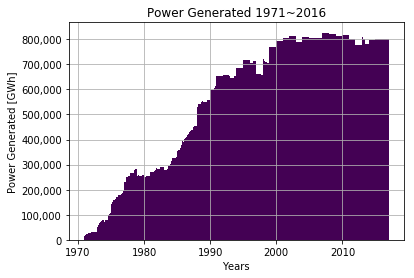
\includegraphics[height=3.5cm]{images/power_gen_cyclus}
      \end{center}
            \caption{Power generated between 1971 and 2016 from the \textsc{Cyclus} simulation}
    \end{figure}
    \column[t]{5cm}
    \begin{figure}[htbp!]
      \begin{center}
        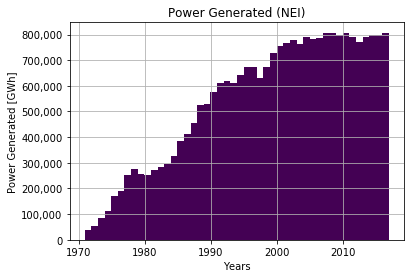
\includegraphics[height=3.5cm]{images/power_gen_nei}
      \end{center}
            \caption{Power generated between 1971 and 2016 as published by the NEI \cite{nei_u.s._2018}}
    \end{figure}
  \end{columns}
\end{frame}
